\section{Plotting Bivariate Data in Python}


Let's use a dataset called Anderson's Iris data to explore bivariate relationships between variables. This data set was published by a a plant biologist named Edgar Anderson in the 1930's (Annals of the Missouri Botanical Garden 23 (3): 457–509) but was made famous by R. A. Fisher who used it to illustrate many of the fundamental statistical methods he developed. The data set consists of four morphometric measurements on specimens of three different iris species.  We'll be using this data set repeatedly in future weeks so familiarize yourself with it.

First, let's use the command line utility |wget| to download the file `iris.cvs' from the course repository to our virtual machine:
\begin{bash}
wget https://github.com/pmagwene/Bio723/raw/master/datasets/iris.csv
\end{bash}

Once the `iris.csv' file is available we can import into Python.  We'll introduce another Python library, called the Pandas, which is an increasingly popular library for statistical analyes in Python.  Pandas share a number of features with R, in particular the use of a data structure called a `data frame' to hold and manipulate multivariate data.
%
\begin{python}
>>> import pandas as pd
>>> iris = pd.read_csv('iris.csv')
>>> iris.shape  # get number and rows and columns in data
(150, 5)
>>> iris.columns  # get the names of the data columns
Index([u'Sepal Length', u'Sepal Width', u'Petal Length', u'Petal Width', u'Species'], dtype='object')

>>> iris.head()  # show first five rows of data set
   Sepal Length  Sepal Width  Petal Length  Petal Width Species
0           5.1          3.5           1.4          0.2  setosa
1           4.9          3.0           1.4          0.2  setosa
2           4.7          3.2           1.3          0.2  setosa
3           4.6          3.1           1.5          0.2  setosa
4           5.0          3.6           1.4          0.2  setosa

>>> iris.tail() # show last five rows of data set
     Sepal Length  Sepal Width  Petal Length  Petal Width    Species
145           6.7          3.0           5.2          2.3  virginica
146           6.3          2.5           5.0          1.9  virginica
147           6.5          3.0           5.2          2.0  virginica
148           6.2          3.4           5.4          2.3  virginica
149           5.9          3.0           5.1          1.8  virginica


>>> iris['Species']  # get the Species column
... lots of output ...
>>> pd.unique(iris['Species'])  # get the unique names in the Species column
\end{python}


\subsection{Bivariate scatter plots}
We'll start with the conventional `variable space' representation of bivariate relationships -- the scatter plot.  
%
\begin{python}
>>> %matplotlib inline  # required in IPython notebook
>>> from pylab import *  # import commonly used plotting functions
>>> scatter(iris['Sepal Length'], iris['Sepal Width'])
>>> xlabel("Sepal Length")
>>> ylabel("Sepal Width")
\end{python}
%
This plots Sepal Length on the x-axis and Petal Length on the y-axis. In many cases it's useful to ensure that the axes of the plot have identifical unit values, so that a one unit change in the x-axis is that as on the y-axis.  Here's how you can ensure that.
%
\begin{python}
>>> gca().set_aspect('equal')
\end{python}
%
In the function above, the |gca()| function called is short for "get current axis", and then we use the |set_aspect| function to make the axes cale equally.


From these plot we can see that these two variables are positively associated (i.e. when one increases the other tends to increase). You will also notice there seem to be distinct clusters of points in the plot. Recall that the iris data set consists of three different species.  Let's regenerate the plot, this time coloring the points according to the species names.
%
First, let's note that the Species column is a categorical variable, which in R we refer to as a `factor'.
%
\begin{python}
>>> setosa = iris[iris["Species"] == 'setosa']
>>> setosa.shape
(50, 5)
>>> versicolor = iris[iris["Species"] == 'versicolor']
>>> virginica = iris[iris["Species"] == 'virginica']
>>> scatter(setosa['Sepal Length'], setosa['Sepal Width'], color='crimson', alpha=0.5)
>>> scatter(versicolor['Sepal Length'], versicolor['Sepal Width'], color='royalblue', alpha=0.5)
>>> scatter(virginica['Sepal Length'], virginica['Sepal Width'], color='forestgreen',alpha=0.5)
\end{python}
%
Let's also label our axes, add a title, and a legend:
%
\begin{python}
>>> xlabel("Sepal Length")
>>> ylabel("Sepal Width")
>>> title("Petal Length vs. Sepal Length")
>>> legend(["I. setosa", "I. versicolor", "I. setosa"], loc="upper right")
\end{python}

% In addition to plotting and coloring the bivariate scatter, we added a title to the plot using the |main| argument and created a legend, using the |legend()| function.  Your output should look like Figure~\ref{fig:irisscatter}.
% %
% \begin{figure}[htbp]
% \centering
% 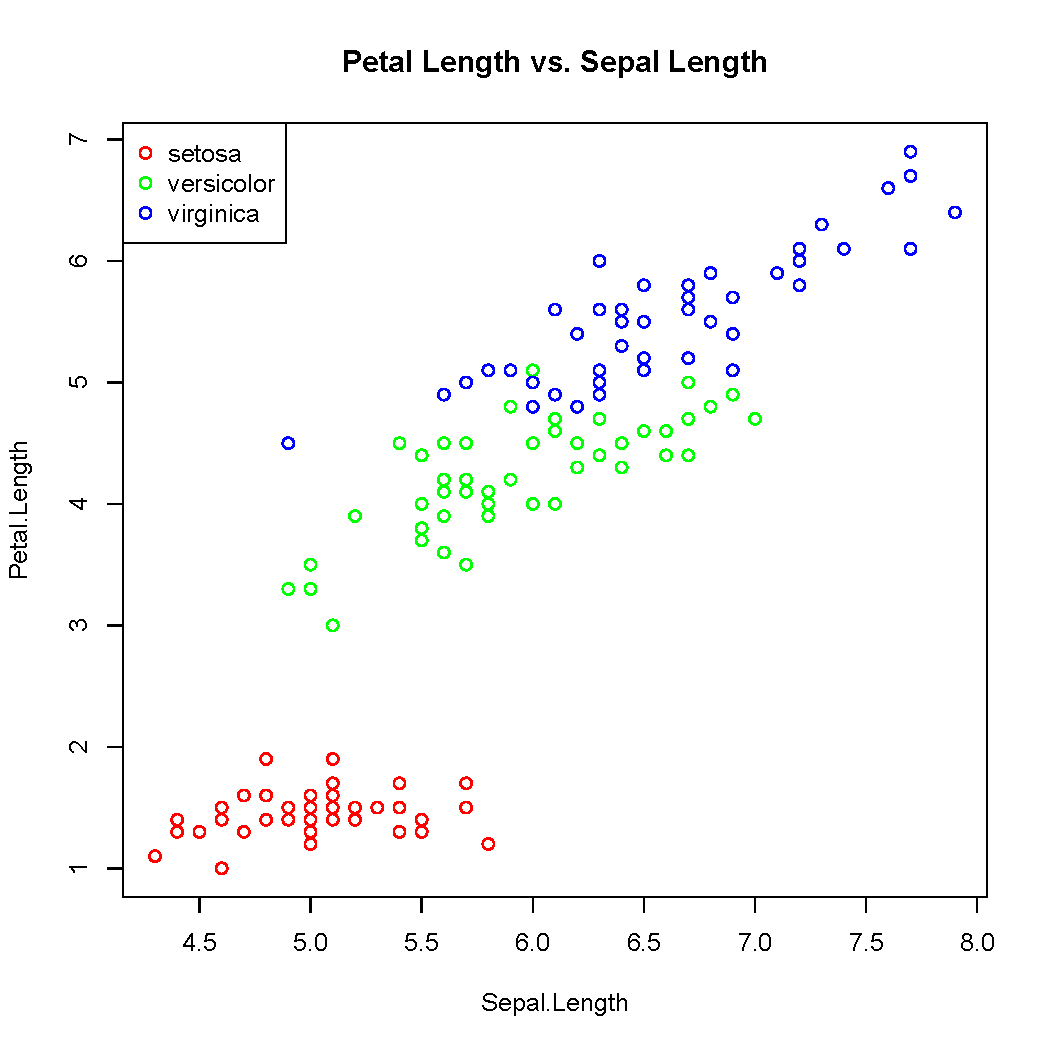
\includegraphics[width=0.4\columnwidth]{./figures/hands-on2/iris-scatter.pdf}
% \caption{Scatter plot created from the iris data set using the \lstinline!plot! function.}
% \label{fig:irisscatter}
% \end{figure}


